\PassOptionsToPackage{sols}{handout}
\documentclass[main]{subfiles}
\setcounterrefbeforedot{chapter}{m-ws4-2}
\setcounterrefafterdot{section}{m-ws4-2}
\addtocounter{section}{-1}
\usepackage{solutions}

\begin{document}

\ifSubfilesClassLoaded{%
  \chaptermark{\chapterfour}
}{}

\section{Relative Growth Rates} \label{ws4-2}

\begin{problemonly}
    \begin{framed}

\textbf{Key Ideas}:

\begin{itemize}[topsep=0pt,partopsep=0pt,parsep=8pt,itemsep=0pt]

\item You should understand what L'H\^{o}pital's Rule implies about
  relative rates of growth of common functions such as logarithms,
  polynomials, and exponentials (for example, that exponentials grow more
  quickly than polynomials).

\item You should know and be able to use the definition of $\ll$. 

\item You should be able to use relative growth rates to streamline your
  reasoning about limits at infinity.

\item You should recognize the form ``$0\cdot\infty$'' as an indeterminate
  form and have a strategy for tackling it.

\end{itemize}
\end{framed}
\end{problemonly}

  \begin{framed}
    \textbf{L'Hôpital's Rule.}  If $\displaystyle \lim_{x \to a}
    \frac{f(x)}{g(x)}$ is a
    \cfitb[\vphantom{$\dfrac{0}{0}$}]{0.3in}{$\bm{{\dfrac{0}{0}}}$} or
    \cfitb[\vphantom{$\dfrac{0}{0}$}]{0.3in}{$\bm{{\dfrac{\infty}{\infty}}}$}
    type of limit, then $\displaystyle \lim_{x
      \to a} \frac{f(x)}{g(x)} =$
    \fitb[\vphantom{$\dfrac{0}{0}$}]{1.25in}{$\bm{\displaystyle \lim_{x \to a}
      \frac{f'(x)}{g'(x)}}$}, if the latter limit exists or is $\pm
    \infty$.
  \end{framed}


\begin{enumerate}
\item
  \begin{enumerate}
  \item
    \begin{problem}[\vfill]
      Sketch the graphs of $\ln x$ and $\sqrt[3]{x}$.  Which do you think
      is larger when $x$ is very large?
    \end{problem}

    \begin{solution}
      If we sketch them individually, they look fairly similar in shape:
      \begin{center}
        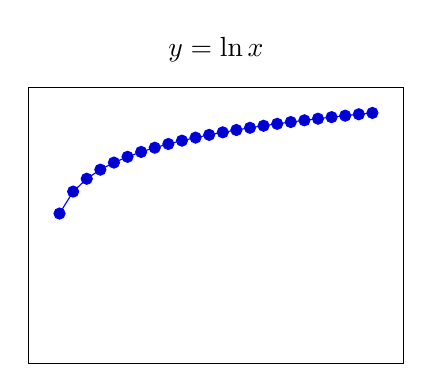
\begin{tikzpicture}
          \begin{axis}[xtick=\empty, ytick=\empty, ymin=-1, width=2.5in,
            height=2in, title={$y = \ln x$}] 
            \addplot+[domain=0:1000] { ln(x)};
          \end{axis}
        \end{tikzpicture}
        \hspace{0.5in}
        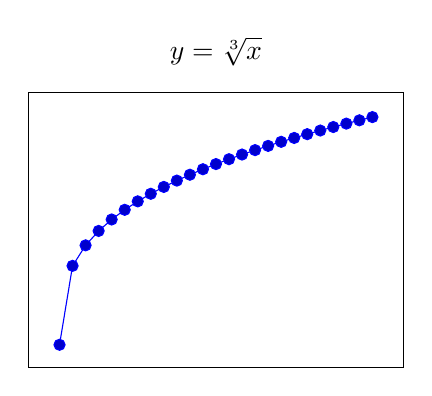
\begin{tikzpicture}
          \begin{axis}[xtick=\empty, ytick=\empty, ymin=-1, width=2.5in,
            height=2in, title={$y = \sqrt[3]{x}$}] 
            \addplot+[domain=0:1000] { x^(1/3) };
          \end{axis}
        \end{tikzpicture}
      \end{center}
    \end{solution}

  \item

    \note{Students might suggest looking at $\displaystyle \lim_{x \to
        \infty} (\ln x - \sqrt[3]{x})$, which is an entirely reasonable
      suggestion.  If this happens, I might use a computer to compare the
      graphs of $x^2$ and something like $x^2 + x$.  If you zoom out, the
      graphs are pretty much indistinguishable, but their difference $\to
      \infty$ as $x \to \infty$.  Looking at the ratio gives a better
      sense of their relative behavior. Given the last problem on the pset
      due today, I think they will look at the ratio.

      If students are surprised that $\ln x \ll \sqrt[3]{x}$, you might
      also want to give them a more concrete idea of why it's true.  For
      example, maybe try plugging something like $x = e^{3000}$ into both
      functions, to see that $\ln \left( e^{3000} \right)$ really is way
      smaller than $\sqrt[3]{e^{3000}}$.}

    \begin{problem}[\vfill]
      How could we use limits to confirm which is larger when $x$ is very
      large? 
    \end{problem}

    \begin{solution}
      We could look at what happens to the ratio $\dfrac{\ln
        x}{\sqrt[3]{x}}$ (or the reciprocal of this) when $x$ gets very
      large.  That is, we look at
      \begin{align*}
        \lim_{x \to \infty} \frac{\ln x}{\sqrt[3]{x}} & \lheq \lim_{x
          \to \infty} \frac{\frac{1}{x}}{\frac{1}{3} x^{-2/3}} \\
        & \nolheq \lim_{x \to \infty} \frac{3}{x^{1/3}} \\
        & \nolheq 0
      \end{align*}
      The fact that this limit is 0 says that, when $x$ is very large,
      $\ln x$ is tiny compared to $\sqrt[3]{x}$.
    \end{solution}

  \item
    \begin{problem}[\vfill\newpage]
      Generalize: If $p$ is any positive number, does $\ln x$ or $x^p$
      grow more quickly?
    \end{problem}

    \begin{solution}
      Again, we can look at what happens to the ratio when $x$ grows
      without bound:
      \begin{align*}
        \lim_{x \to \infty} \frac{\ln x}{x^p} & \lheq \lim_{x \to
          \infty} \frac{\frac{1}{x}}{p x^{p-1}} \\
        & \nolheq \lim_{x \to \infty} \frac{1}{p x^p} \\
        \intertext{Since $p > 0$, $x^p \to \infty$ as $x \to \infty$, so
          this limit is}
        & \nolheq 0
      \end{align*}
      Therefore, \fbox{$x^p \gg \ln x$}.
    \end{solution}

  \end{enumerate}

\end{enumerate}

  \begin{framed}
    Suppose $f(x)$ and $g(x)$ are functions that are both positive when
    $x$ is large.  We say that $g(x)$ \uline{grows more quickly than}
    $f(x)$, written $g(x) \gg f(x)$, if $\displaystyle \lim_{x \to
      \infty} \frac{f(x)}{g(x)} = \cfitb{0.25in}{0}$ (or, equivalently,
    if $\displaystyle \lim_{x \to \infty} \frac{g(x)}{f(x)} =
    \cfitb{0.25in}{\infty}$).
  \end{framed}


\begin{enumerate}[resume]
\item 
  \begin{enumerate}
  \item
    \begin{problem}[\vfill]
      Does $1.001^x$ or $x^2$ grow more quickly?  Use the limit definition
      of $\gg$ to support your answer. 
    \end{problem}

    \begin{solution}
      To answer this, we should calculate either $\displaystyle \lim_{x
        \to \infty} \frac{1.001^x}{x^2}$ or $\displaystyle \lim_{x \to
        \infty} \frac{x^2}{1.001^x}$; it doesn't matter which.
      \begin{align*}
        \lim_{x \to \infty} \frac{x^2}{1.001^x} & \lheq \lim_{x \to
          \infty} \frac{2x}{1.001^x \ln 1.001} \\
        & \lheq \lim_{x \to
          \infty} \frac{2}{1.001^x (\ln 1.001)^2} \\
        & \nolheq 0,
      \end{align*}
      so $\boxed{x^2 \ll 1.001^x}$.
    \end{solution}

  \item

    \note{This is just one more concrete example to help them build
      their intuition for the general case.}

    \begin{problem}[\vfill]
      Does $1.0001^x$ or $3x^3 + 7x + 5$ grow more quickly?  Use the
      limit definition of $\gg$ to support your answer.
    \end{problem}

    \begin{solution}
      Let's look at what happens to the ratio when $x$ grows without
      bound:
      \begin{align*}
        \lim_{x \to \infty} \frac{3x^3 + 7x + 5}{1.0001^x} & \lheq
        \lim_{x \to \infty} \frac{27 x^2 + 7}{1.0001^x \ln 1.0001} \\
        & \lheq \lim_{x \to \infty} \frac{54 x}{1.0001^x (\ln 1.0001)^2}
        \\
        & \lheq \lim_{x \to \infty} \frac{54}{1.0001^x (\ln 1.0001)^3}
        \\
        & \nolheq 0,
      \end{align*}
      so $\boxed{1.0001^x \gg 3x^3 + 7x + 5}$. 
    \end{solution}

  \item

    \note{An important point here is that, if $b < 1$, then $b^x$ does not
      grow at all, so $b^x \ll P(x)$.}

    \begin{problem}[\vfill]
      Generalize: If $P(x)$ is a polynomial with a positive leading
      coefficient\footnote{The \uline{leading coefficient} of a polynomial
        is the coefficient of the highest degree term.  For instance, the
        leading coefficient of $-2x^4 + x^3 + 7x^2$ is $-2$.} and $b > 0$,
      does $b^x$ or $P(x)$ grow more quickly?  (Does it depend on the
      particular polynomial, or on the value of $b$?)
    \end{problem}

    \begin{solution}
      First, if $b \leq 1$, then $b^x$ does not grow as $x \to \infty$,
      so in that case $b^x \ll P(x)$. 

      If $b > 1$, both $b^x$ and $P(x)$ grow without bound as $x \to
      \infty$, so we can look at their ratio to understand which grows
      faster:
      \begin{align*}
        \lim_{x \to \infty} \frac{P(x)}{b^x} & \lheq \lim_{x \to \infty}
        \frac{P'(x)}{b^x \ln b} \\
        \intertext{If $P(x)$ has degree $> 1$, then this is still an
          $\frac{\infty}{\infty}$ limit:}
        & \lheq \lim_{x \to \infty} \frac{P''(x)}{b^x (\ln b)^2} \\
        \intertext{We can continue using L'H\^opital's Rule in this way;
          eventually, we will have differentiated the numerator enough
          times that it's just a number, while the denominator will
          still be $b^x (\ln b)^{\text{some power}}$, so the limit will
          be} %
        & \nolheq 0
      \end{align*}
      So, we conclude: \fbox{if $b \leq 1$, then $b^x \ll P(x)$; if $b >
        1$, then $b^x \gg P(x)$}. 
    \end{solution}

  \end{enumerate}

\item 
  \begin{problem}[\nstretch{0.3}]
    All of the following functions increase without bound as $x \to
    \infty$.  Put them in order from slowest growing to fastest.
    \[ 1.01^x \qquad 3^{2x} \qquad 2^{3x} \qquad \sqrt[7]{x} \qquad
    x^{1,000,000} \qquad \log_7 x \qquad x \ln x \]
  \end{problem}

  \begin{solution}
    First, as we've seen already, logs grow more slowly than positive
    powers of $x$, and positive powers of $x$ grow more slowly than
    exponentials whose base is $> 1$.  So, we can separate these into a
    few groups:
    \[ \underbrace{\log_7 x}_{\text{log}} \qquad \ll \qquad
    \underbrace{\sqrt[7]{x} \qquad x^{1,000,000}}_{\text{positive powers
        of $x$}} \qquad \ll \qquad \underbrace{1.01^x \qquad 3^{2x}
      \qquad 2^{3x} }_{\text{exponentials with base $> 1$}}\] (And then
    we still have to figure out where $x \ln x$ fits.)
    It's clear that $\sqrt[7]{x} = x^{1/7}$ grows more slowly than
    $x^{1,000,000}$.  To compare the exponentials, it's convenient to
    rewrite them so that they all have an exponent of just $x$: $3^{2x}
    = (3^2)^x = 9^x$ and $2^{3x} = (2^3)^x = 8^x$.  Since $1.01^x
    \ll 8^x \ll 9^x$, we can now order all of the expressions except for
    $x \ln x$:
    \[ \log_7 x \ll \sqrt[7]{x} \ll x^{1,000,000} \ll 1.01^x \ll 2^{3x}
    \ll 3^{2x}.\] Since just $x$ grows faster than $\sqrt[7]{x}$, $x \ln
    x$ must also grow faster than $\sqrt[7]{x}$ (because $x \ln x > x$
    when $x$ is big).  On the other hand, since $\ln x$ grows more
    slowly than $x$, $x \ln x$ should grow more slowly than $x \cdot x =
    x^2$, so it certainly must grow more slowly than $x^{1,000,000}$.
    This gives us the final ordering
    \[ \boxed{\log_7 x \ll \sqrt[7]{x} \ll x \ln x \ll x^{1,000,000} <
      1.01^x \ll 2^{3x} \ll 3^{2x}}.\]
  \end{solution}

\item  \emph{Using relative growth rates to reason about limits at
    infinity.}

  \begin{enumerate}
  \item

    \note{Here, I just want to remind them that they've seen the idea that
      they only need to look at the fastest-growing terms in the numerator
      and denominator, $2x^3$ and $5x^3$.  In this case, we can justify it
      easily with algebra.}

    \begin{problem}[\vfill]
      Evaluate $\displaystyle \lim_{x \to \infty} \frac{2x^3 +
        \sqrt{x}}{5x^3 + 4 x^2 + 4}$.
    \end{problem}

    \begin{solution}
      As you saw in Math Ma, only the fastest growing term in the
      numerator and the fastest growing term in the denominator are
      important: $\displaystyle \lim_{x \to \infty} \frac{2x^3 +
        \sqrt{x}}{5x^3 + 4 x^2 + 4} = \lim_{x \to \infty}
      \frac{2x^3}{5x^3} = \boxed{\frac{2}{5}}$.
    \end{solution}

  \item

    \note{I'll let them know that the same principle applies even with
      more complicated functions.}

    \begin{problem}[\vfill]
      Apply the same idea to evaluate $\displaystyle \lim_{x \to \infty}
      \frac{\ln x + \pi x^{0.1} + e^{-x}}{\sqrt[10]{7x} + \frac{1}{x}}$.
    \end{problem}

    \begin{solution}
      In the sum $\ln x + \pi x^{0.1} + e^{-x}$, $\pi x^{0.1}$ is the
      fastest growing term.  In the sum $\sqrt[10]{7x} + \frac{1}{x}$,
      $\sqrt[10]{7x}$ is the faster growing term.  Therefore, the given
      limit is equal to $\displaystyle \lim_{x \to \infty} \frac{\pi
        x^{0.1}}{\sqrt[10]{7x}}$, which we can rewrite as $\displaystyle
      \lim_{x \to \infty} \frac{\pi x^{0.1}}{\sqrt[10]{7} \sqrt[10]{x}} =
      \boxed{\frac{\pi}{\sqrt[10]{7}}}$.
    \end{solution}

  \end{enumerate}

\item  

  Evaluate the following limits.

  \begin{enumerate}

  \item

    \note{It is common for students to just want to keep $x^2$ in the
      numerator because $x^2 \ln x \gg x^2$.}

    \begin{problem}[\vfill]
      $\displaystyle \lim_{x \to \infty} \frac{x^2 \ln x}{3 x^2 + 17}$
    \end{problem}

    \begin{solution}
      In the sum $3x^2 + 17$, $3x^2$ is the faster growing term, so this
      limit is equal to $\displaystyle \lim_{x \to \infty} \frac{x^2 \ln
        x}{3 x^2} = \lim_{x \to \infty} \frac{\ln x}{3} = \boxed{\infty}$.
    \end{solution}

  \item
    \begin{problem}[\vfill]
      $\displaystyle \lim_{x \to -\infty} \frac{e^x + x^2}{7x^3 + 5}$
    \end{problem}

    \begin{solution}      
      As $x \to -\infty$, $e^x \to 0$, so $x^2$ is the faster growing term
      in the sum $e^x + x^2$.  In the sum $7x^3 + 5$, $7x^3$ is the faster
      growing term, so the given limit is equal to $\displaystyle \lim_{x
        \to -\infty} \frac{x^2}{7x^3} = \lim_{x \to -\infty} \frac{1}{7x}
      = \boxed{0}$.
    \end{solution}

  \item

    \begin{problem}[\vfill\newpage]
      $\displaystyle \lim_{x \to \infty} \frac{x^2 + 1.01^x + 7 \sin
        x}{\ln x + \sqrt{x} + 1.02^x}$
    \end{problem}

    \begin{solution}
      In the sum $x^2 + 1.01^x + 7 \sin x$, $1.01^x$ is the fastest
      growing term (we know $1.01^x \gg x^2$, and $7 \sin x$ doesn't
      really grow; it just oscillates between $-7$ and $7$, so $1.01^x$
      definitely grows faster than $7 \sin x$).  In the sum $\ln x +
      \sqrt{x} + 1.02^x$, $1.02^x$ is the fastest growing term.  So, the
      given limit is equal to $\displaystyle \lim_{x \to \infty}
      \frac{1.01^x}{1.02^x} = \lim_{x \to \infty} \left( \frac{1.01}{1.02}
      \right)^x = \boxed{0}$. 
    \end{solution}

  \end{enumerate}

  % \item

  % \begin{problem}[\nstretch{1.5}]
  %   Evaluate $\displaystyle \lim_{x \to 0^+} \sqrt{x} e^{1/x}$.  What form
  %   is this limit?
  % \end{problem}

  % \begin{solution}
  %   This is a $0 \cdot \infty$ limit.  We can rewrite it as
  %   \begin{align*}
  %     \lim_{x \to 0^+} \frac{e^{1/x}}{x^{-1/2}} & \lheq \lim_{x \to 0^+}
  %     \frac{e^{1/x} \left( - \frac{1}{x^2} \right)}{- \frac{1}{2}
  %       x^{-3/2}} \\
  %     & \nolheq \frac{2 e^{1/x}}{\sqrt{x}} \\
  %     \intertext{Now, the numerator $\to \infty$ while the denominator
  %       $\to 0^+$, so the limit is equal to:}
  %     & \nolheq \boxed{\infty}
  %   \end{align*}
  % \end{solution}

\item 

  \note{Matt note - this is transitioning us back to exploring indeterminate forms. 
  
  I mostly want them to develop their intuition here about what an
    indeterminate form is.}

  Are limits of the following forms indeterminate or not?

  \begin{enumerate}
  \item
    \begin{problem}[\vfill]
      ``$\displaystyle \frac{0}{\infty}$''
    \end{problem}

    \begin{solution}
      This is \fbox{not indeterminate}; it's just always 0.  That is, if
      $\displaystyle \lim_{x \to a} f(x) = 0$ and $\displaystyle \lim_{x
        \to a} g(x) = \infty$, then $\displaystyle \lim_{x \to a}
      \frac{f(x)}{g(x)} = 0$.
    \end{solution}

  \item
    \begin{problem}[\vfill]
      ``$0 \cdot \infty$''
    \end{problem}

    \begin{solution}
      This \fbox{is indeterminate}.  Just knowing that $\displaystyle
      \lim_{x \to a} f(x) = 0$ and $\displaystyle \lim_{x \to a} g(x)
      = \infty$ doesn't tell us the value of $\displaystyle \lim_{x \to a}
      f(x) \cdot g(x)$.  Here are some examples:
      \begin{itemize}
      \item $\displaystyle \lim_{x \to \infty} \tfrac{1}{x} = 0$,
        $\displaystyle \lim_{x \to \infty} 7x =
        \infty$, and $\displaystyle \lim_{x \to \infty}
        \tfrac{1}{x} \cdot 7x = 7$.  (Of course, if we changed the 7 to
        any other value, we could get a 
        ``$0 \cdot \infty$'' limit with that value.)
      \item $\displaystyle \lim_{x \to \infty} \tfrac{1}{x} = \infty$,
        $\displaystyle \lim_{x \to \infty} x^2 = \infty$, and
        $\displaystyle \lim_{x \to \infty}
        \tfrac{1}{x} \cdot x^2 = \infty$. 
      \end{itemize}
    \end{solution}

  \item
    \begin{problem}[\vfill]
      ``$\infty \cdot \infty$''
    \end{problem}

    \begin{solution}
      This is \fbox{not indeterminate}; such a limit is always $\infty$.  That
      is, if $\displaystyle \lim_{x \to a} f(x) = \infty$ and
      $\displaystyle \lim_{x \to a} g(x) = \infty$, then $\displaystyle
      \lim_{x \to a} f(x) g(x) = \infty$. 
    \end{solution}

  \end{enumerate}


\note{Matt note - This is here to set up next class. The main thing to leave them with is that we have not seen all types of indeterminate forms yet.}

  \item Evaluate the limits below.
\begin{multicols}{3}
\begin{enumerate}



  \item $\lim\limits_{x\to\infty} \left(\frac{1}{2}\right)^x\solonly{=0}$

  \item $\lim\limits_{x\to\infty} (0.99999999)^x\solonly{=0}$

  \item $\lim\limits_{x\to\infty} (1.0000001)^x\solonly{=\infty}$

\end{enumerate}
\end{multicols}

\begin{solution}
\begin{enumerate}

  \item This limit is zero because the base of the exponent is between $0$ and $1$,
    so this is exponential decay. As $x$ increases, $x=1$, $2$, $3$, \dots , we
    multiply by $\frac{1}{2}$ over and over, and so $\left(\frac{1}{2}\right)^x$
    becomes smaller and smaller, closer and closer to $0$.

  \item This limit is zero because the base of the exponent is between $0$ and $1$,
    so this is exponential decay. As $x$ increases, $x=1$, $2$, $3$, \dots , we
    multiply by $0.99999999$ over and over, and so $(0.99999999)^x$
    becomes smaller and smaller, closer and closer to $0$, albeit more slowly than
    $\left(\frac{1}{2}\right)^x$.

  \item This limit is $\infty$ because the base of the exponent is greater than
    $1$, so this is exponential growth. As $x$ increases, $x=1$, $2$, $3$, \dots ,
    we multiply by $1.0000001$ over and over, and so $(1.0000001)^x$
    becomes larger and larger, growing without bound.

\end{enumerate}
\end{solution}


\pspace{\stretch{0.5}}

\note{Matt note - we are going to start next class with evaluating this limit.}

\item
\begin{problem}[\nstretch{1.5}]
  Consider the limit $\lim\limits_{x\to\infty} (1+\frac{1}{x})^x$. Can you 
  look at this and easily determine the value?
\end{problem}

\begin{solution}
  This limit is not as easily deduced as the previous ones. On the one hand, we 
  have numbers greater than $1$ being raised to larger and larger powers. This
  suggests that the limit could be $\infty$. On the other hand, as $x$ increases,
  $x=1$, $2$, $3$, \dots , we multiply by numbers that are closer and closer to
  $1$, which means $(1+\frac{1}{x})^x$ grows more and more slowly and may
  eventually approach some fixed number.
  
\end{solution}

\end{enumerate}

\end{document}